\title{Scalable Parallel-in-Time Integration \\ \Large{Acoustics in Expanding Volumes}}
\author{
    Nathan Chapman\textsuperscript{1}, Andy Piacsek\textsuperscript{2} \\
    \textsuperscript{1}Department of Computer Science, Central Washington University \\
    \textsuperscript{2}Department of Physics, Central Washington University
}
\date{\today}

\maketitle

\section*{Introduction}
	\begin{itemize}
		\item Work in Progress
		\item This work is a work in progress and is expected to be completed in the Spring!
	\end{itemize}

\subsection*{The Equations of Motion and Causality}
The equations of motion (EoM) are at the heart of physics:
\[
\sum_i \vec{F}_i = m\vec{a}.
\]

\begin{itemize}
	\item Numerical methods for solving these equations have historically been sequential to follow causality. 
	\item This sequential nature has limited their ability to benefit from parallelism. 
	\item But what if they could?
\end{itemize}

\section*{Acoustics in Expanding Volumes}
Wave $\psi(t, \vec{x})$ is defined by its density $n$ and phase $\theta$ as:
\[
\psi(t, \vec{x}) = \sqrt{n_0 + \Delta n(t, \vec{x})} e^{i(\theta_0 + \Delta \theta(t, \vec{x}))}.
\]

The wave equation for an expanding volume is:
\[
\partial_t^2 \theta - \frac{\dot{a}}{a} \partial_t \theta - a c_0^2 \nabla^2 \theta = 0.
\]

Applying a spectral decomposition in space:
\[
\tilde{\theta}_{\vec{k}} = \mathcal{F}(\Delta \theta)(t, \vec{k}), \quad \text{for } k < k_c(t),
\]
results in:
\[
\partial_t^2 \tilde{\theta}_{\vec{k}} - \frac{\dot{a}}{a} \partial_t \tilde{\theta}_{\vec{k}} - a c_0^2 k^2 \tilde{\theta}_{\vec{k}} = 0.
\]

For each wave number $k$:
\[
\partial_t^2 \tilde{\theta}_{\vec{k}} - \frac{\dot{a}}{a} \partial_t \tilde{\theta}_{\vec{k}} - a c_0^2 k^2 \tilde{\theta}_{\vec{k}} = 0, \quad \text{with initial conditions: }
\]
\[
\tilde{\theta}_{\vec{k}}(0) = \tilde{\theta}_{\vec{k}_0}, \quad \partial_t \tilde{\theta}_{\vec{k}}(0) = -U_0 n_{\vec{k}_0} / \hbar.
\]

The method of lines approach results in ordinary differential equations for each wave number.

\section*{Methods}
\subsection*{Parallel-in-Time Integration and the Parareal Algorithm}
Parallel-in-time integration attempts to solve initial value problems (IVPs) in parallel. Notable algorithms include:
\begin{itemize}
    \item Parareal,
    \item Multigrid Reduction in Time (MGRIT),
    \item Parallel Full Approximation Scheme in Space and Time (PFASST), and others.
\end{itemize}

\subsubsection*{The Four Core Steps of the Parareal Algorithm}
\begin{enumerate}
    \item \textbf{Prepare the subproblems:}
    Given an initial value problem $P$:
    \[
    \mathcal{L}(t, u, \partial_t u, \partial_t^2 u) = f(t), \quad u(0) = u_0, \quad \partial_t u(0) = v_0,
    \]
    where $D = [T, T + \Delta T]$. Choose the number of subproblems $N$ (suggested: the number of compute cores). Partition the time domain $D$ into subdomains $D_p$:
    \[
    D_p = [T + p / N \Delta T, T + (p + 1) / N \Delta T] = [T_p, T_{p+1}].
    \]
    Use a coarse propagator $\mathcal{C}_0$ to compute initial solutions $\{u_p^0\}_p$, $\{v_p^0\}_p$.

    \item \textbf{Solve each subproblem in parallel:}
    Use a coarse propagator $\mathcal{C}$ (e.g., Runge-Kutta 2 with a large time step) and a fine propagator $\mathcal{F}$ (e.g., Velocity-Verlet with a small time step). Solve each subproblem $p$ in parallel.

    \item \textbf{Correct:}
    Compute corrections for the coarse solutions using:
    \[
    \eta_p^i = \mathcal{F} u_p^i (T_{p+1}) - \mathcal{C} u_p^i (T_{p+1}),
    \]
    and apply corrections sequentially:
    \[
    u_{p+1}^i(T_{p+1}) = u_p^i(T_{p+1}) + \eta_p^i.
    \]

    \item \textbf{Iterate:}
    Repeat the process for updated initial values until convergence, e.g.:
    \[
    |u_p^i - u_p^{i-1}| < \epsilon \quad \forall p \leq N.
    \]
\end{enumerate}

\subsection*{GPU and Distributed Computing}
\textbf{GPU Parallelism:} GPUs, with their thousands of cores, allow solving 15,000+ subproblems concurrently, greatly enhancing accuracy compared to CPU parallelism, which typically supports only $\sim$10 cores.

\textbf{Distributed Computing:} Distributed computing frameworks like MPI enable computations across multiple machines, allowing all wave numbers to be solved simultaneously, scaling efficiently to clusters and supercomputers.

\section*{Results}
\subsection*{Some Basic Results}
\begin{figure}[h!]
    \centering
    % 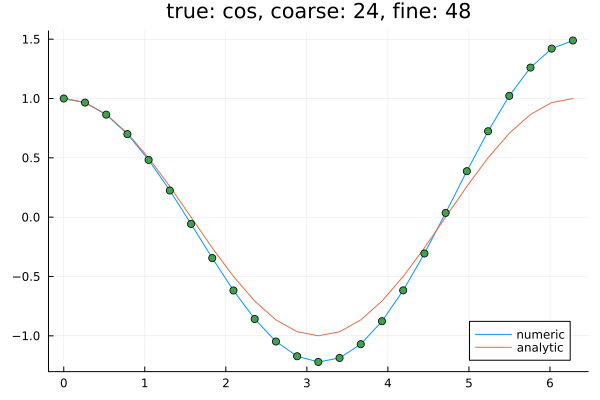
\includegraphics[width=0.7\textwidth]{figures/cos_24_48.svg}
    \caption{Local CPU-based solution to $u''(t) = -u(t), u(0) = 1, u'(0) = 0$, evaluated on 24 threads.}
\end{figure}

\section*{Conclusion}
\begin{itemize}
    \item Equations of motion can now benefit from parallel solvers.
    \item Certain problems are well-suited to a divide-and-conquer approach.
    \item Problems with "doubly parallel" characteristics can leverage both local and distributed parallelism, achieving significant computational efficiency.
    \item These advancements pave the way for modeling acoustics in expanding volumes.
\end{itemize}
